\section{Overview}\label{sec:overview}
Given a 2D expanded layout of a carton, our system allow users to explore the shape and structure of corresponding models. Figure~\ref{fig:overview} is our construction algorithm overview. Given a 2D layout Figure~\ref{fig:overview}(a), its 2D mesh Figure~\ref{fig:overview}(b) is created by ignoring the holes in the plane, and the initial 3D model Figure~\ref{fig:overview}(c) is constructed by given a specific angle to each fold edge which will be explained later in section~\ref{sec:initialization}, then the final model Figure~\ref{fig:overview}(d) is finally built through the optimization based on the information acquired from user interaction. 

\begin{figure}
	\centering
	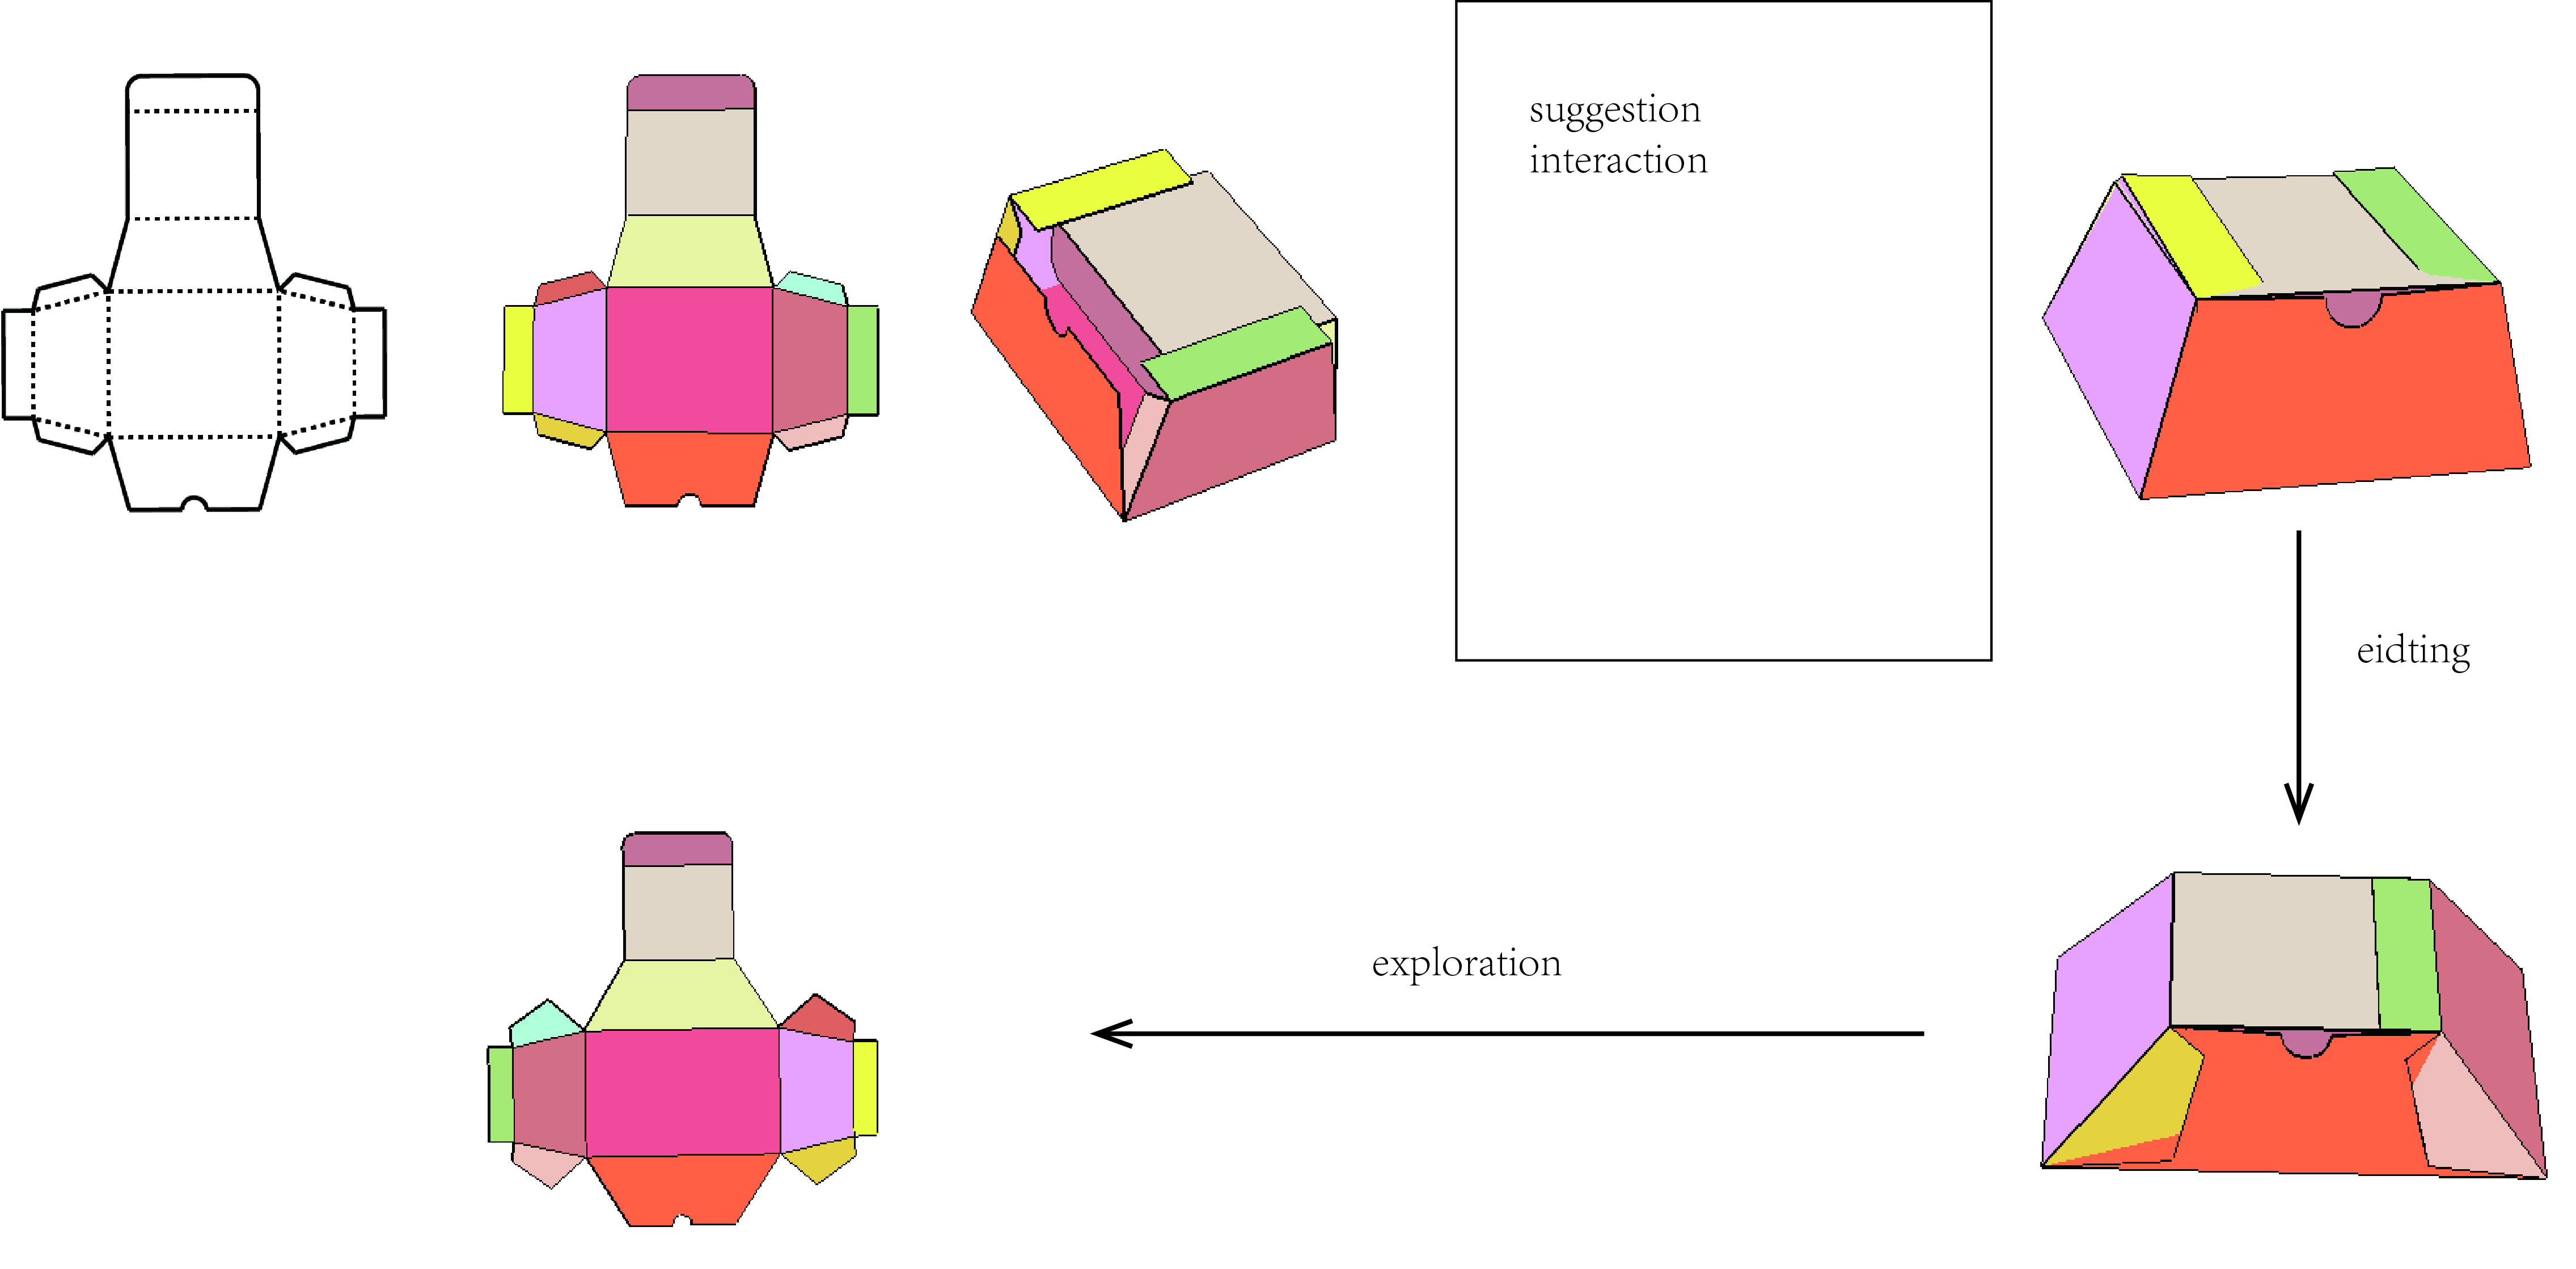
\includegraphics[width=0.9\textwidth]{images/overview.jpg}
	\caption{Given a 2D layout(a), we first create its 2D mesh(b), and by given a specific angle to each fold edge, we can construct the initial 3D model(c), the final model(d) is finally built through the optimization based on the information acquired from user interaction.}
	\label{fig:overview}
\end{figure} 

To formulate our problem, we assume that every plane is rigid which means the interior angle in each plane stays the same, but planes can be bent during folding. Furthermore, planes are connected by hinges at the boundary of patches, and the planar layout has its front and back.